% !TeX encoding = UTF-8
% !TeX program = xelatex
% !TeX spellcheck = <none>

\documentclass[degree=project, degree-type=project]{thuthesis}
\usepackage{mathtools}

% 论文基本配置,加载宏包等全局配置
\thusetup{
    output = electronic,
    title  = {随机过程在机器学习中的应用},
    author  = {肖文韬},
    studentid = {2020214245},
    course = {随机过程},
    include-spine = false,
}

\usepackage{float}
\usepackage[sort]{natbib}
\bibliographystyle{thuthesis-numeric}
\graphicspath{{figures/}}

\begin{document}

\maketitle

\frontmatter
\begin{abstract}
	工程系统的设计是为了在部件特性和运行条件不确定的情况下良好地运行。
	在某些情况下,系统运行中有意引入了不确定性。
	了解如何建立不确定性模型以及如何分析其影响是——或者说应该是——工程师教育的一个重要部分。
	随机性是我们设计的所有系统的一个关键因素。
	通信系统被设计为补偿噪声;互联网路由器是为了吸收流量波动而设计的;建筑物必须能抵抗地震时不可预测的振动;配电网承载着不可预知的负荷;集成电路的制造步骤会出现不可预知的变化;搜索基因是在未知的字符串中寻找模式。
	本文主要聚焦于数值方法在机器学习领域。
	随机过程在机器学习领域的应用包括但不限于:
	\begin{enumerate}
		\item 高斯过程
		\item 马尔可夫过程
	\end{enumerate}
	本文主要将围绕上述两个主题总结和讨论随机过程在机器学习领域的应用。

	\thusetup{
		keywords = {随机过程, 高斯过程,马尔可夫过程},
	}
\end{abstract}

\tableofcontents
\mainmatter

\chapter{概述}
\label{chap:intro}
随机过程是一种数学工具,用于建立与时间有关的随机现象的模型。
随机过程在多个领域都有应用,只要认识到物理、生物、金融等系统中随机发生的事件的随机性和不可预测性的作用,随机过程就能发挥作用。
例如,在物理学的应用中可以提到相变、原子发射现象等。在生物学中,生命体的时间行为常常受到随机性的影响,至少在观察者只能获得部分信息的情况下是如此。后面这一点很重要,因为它把随机性的概念和信息的概念联系起来了:对一个观察者来说看似随机的东西,对另一个拥有更多信息的观察者来说,可能不是随机的。举例来说,想想观察汽车在十字路口转弯的明显随机行为与汽车司机的观点,他们每个人都是按照自己的决定行事。在金融学中,对时间相关的随机现象进行建模的重要性是相当明显的,因为没有人能够对风险资产的未来走势做出明确的预测。随机建模的具体结果在于计算期望值或预期值,这往往比概率值本身更有用。例如,一个平均或预期寿命,可能比一个(小)违约概率更容易解释。随机系统的长期统计行为,也涉及到期望值的估计,是一个相关的问题。

我们将在第~\ref{chap:gp}章介绍高斯过程的应用,然后在第~\ref{chap:hmm}章介绍马尔可夫过程及其应用。
最后在第~\ref{chap:conclusion}总结。

\chapter{高斯过程}
\label{chap:gp}

高斯过程是多变量高斯随机变量对无限(离散或连续)时间集的扩展。
高斯过程已经被大量应用于各种不同的领域,并且有非常多关于各种性质的深入理论分析。
高斯过程模型经常被用来解决困难的机器学习问题。
它之所以吸引人,是因为其灵活的非参数性质和计算的简单性。
在贝叶斯框架内处理,通过高斯过程可以实现非常强大的统计方法,这些方法提供了我们预测中不确定性的有效估计,以及作为非线性优化问题的通用模型选择程序。
在本章节中,我们旨在介绍高斯过程与机器学习相关的特征。

\section{高斯过程在回归任务上的应用}

回归任务可以概括为:给定一个因变量在自变量 $x$ 的某些值上的有噪声的观测值,对于一个新的值 $x_*$,我们对因变量的最佳估计是什么?

如果我们预期基本函数 $f(x)$ 是线性的,并且可以对输入数据做出一些假设,我们可以使用最小二乘法来拟合一条直线(线性回归)。
此外,如果我们怀疑 $f(x)$ 也可能是二次方、三次方,甚至是非多项式,我们可以利用模型选择原则在各种可能性中进行选择。
高斯过程回归是一种比这更巧妙的方法。
高斯过程不是宣称 $f(x)$ 与某些特定模型有关(例如 $f(x)=mx+c$ ),而是通过让数据更清楚地 “说话”,倾斜但严格地表示 $f(x)$。
高斯过程回归仍然是监督学习的一种形式,但训练数据的利用方式更巧妙。
因此,高斯过程回是一个不太 “参数化” 的工具。
然而,它并不是完全自由形式的,如果我们不愿意对 $f(x)$ 做出哪怕是基本的假设,那么就应该考虑更通用的技术,包括那些以最大熵原则为基础的技术。

高斯过程将多变量高斯分布扩展到无限维度。
形式上,高斯过程产生的数据位于某个领域,使范围内的任何有限子集都遵循多变量高斯分布。
现在,任意数据集中的 $n$ 个观测值,$y = \{y_1, \cdots, y_n\}$,总是可以想象成从某个多变量高斯分布中采样的一个点。
因此,往后推,这个数据集可以和高斯过程配对。
因此,高斯过程是普适的,因为它们的条件很简单。

很多时候,人们假设这个对应的高斯过程的平均数在任何地方都是零。
在这种情况下,将一个观测值与另一个观测值联系起来的只是协方差函数 $k(x, x^\prime)$。一个流行的选择是 "平方指数":
\begin{equation}\label{cov}
k(x, x^\prime) = \sigma_f^2 \left[\frac{- (x - x^\prime)^2}{2l^2}\right]
\end{equation}
其中,最大允许协方差定义为 $\sigma_f^2$ 对于覆盖 $y$ 轴广泛范围的函数来说,这个值应该很高。
如果 $x \approx x^\prime$, $k(x, x^\prime)$ 将会接近这个最大值,也就是说 $f(x)$ 与 $f(x^\prime)$ 非常地相关。
这样就是函数 $f$ 会比较平滑。
因此,例如,在新的 $x$ 值的插值过程中,远距离观测的影响将可以忽略不计。
这种分离的影响有多大,将取决于长度参数 $l$,所以公式~\ref{cov}中有很大的灵活性。

不过这样灵活性还不够:数据通常也是有噪声的,来自测量误差等。
每个观测值 $y$ 都可以被认为是通过高斯噪声模型与基本函数 $f(x)$ 有关:
\begin{equation}
y = f(x) + \mathcal{N}(0, \sigma_n^2)
\end{equation}

对于那些曾经做过回归的人来说应该很熟悉。
回归就是寻找 $f(x)$,我们可以采用了一种新颖的方法,将噪声折叠到 $k(x, x^\prime)$:
\begin{equation}\label{cov_g}
k(x,x^\prime) = \sigma_f^2 \exp\left[\frac{-(x-x^\prime)^2}{2l^2}\right] + \sigma_n^2 \delta(x,x^\prime)
\end{equation}
其中 $\delta$ 是 Kronecker delta 函数。

为了准备高斯过程回归,我们使用公式~\ref{cov_g}计算所有点的可能组合,得到:
\begin{align}
	K&=\left[\begin{array}{cccc}
	k\left(x_{1}, x_{1}\right) & k\left(x_{1}, x_{2}\right) & \cdots & k\left(x_{1}, x_{n}\right) \\
	k\left(x_{2}, x_{1}\right) & k\left(x_{2}, x_{2}\right) & \cdots & k\left(x_{2}, x_{n}\right) \\
	\vdots & \vdots & \ddots & \vdots \\
	k\left(x_{n}, x_{1}\right) & k\left(x_{n}, x_{2}\right) & \cdots & k\left(x_{n}, x_{n}\right)
	\end{array}\right] \\
	K_{*} &= [k(x_*, x_1), \cdots, k(x_*, x_n)] \\
	k_{**} &= k(x_*, k_*)
\end{align}

因为高斯过程模型的核心假设就是数据可以使用多维高斯分布的简单形式来表示:
\begin{equation}
\left[\begin{array}{c}
\mathbf{y} \\
y_{*}
\end{array}\right] \sim \mathcal{N}\left(\mathbf{0},\left[\begin{array}{cc}
K & K_{*}^{\mathrm{T}} \\
K_{*} & K_{* *}
\end{array}\right]\right)
\end{equation}

我们感兴趣的的就是条件概率 $p(y_* | \boldsymbol{y})$:给定数据,当前 $y_*$ 最有可能的预测值是多少?这个条件概率经过推导可以表示为一个高斯分布:
\begin{equation}
	y_* | \boldsymbol{y} \sim \mathcal{N}(K_* K^{-1}\boldsymbol{y}, k_{**} - K_*K^{-1}K_*^T)
\end{equation}

对 $y_*$ 的最佳估计当然就是该分布的均值:
\begin{equation}
\bar{y}_* = K_* K^{-1}\boldsymbol{y}
\end{equation}

对于这里的高斯过程回归,我们需要解决的是三个参数的取值:$\boldsymbol{\theta} = \{l, \sigma_n, \sigma_f\}$。
为了得到最大的 $p(\boldsymbol{\theta}| \boldsymbol{x}, \boldsymbol{y})$ 时对应的参数,我们可以使用最大后验估计,通过贝叶斯公式,我们只需要最大化后验概率:
\begin{equation}
\log p(\boldsymbol{y}|\boldsymbol{x},\boldsymbol{\theta}) = -\frac{1}{2} \boldsymbol{y}^T K^{-1} \boldsymbol{y} - \frac{1}{2} \log |K| - \frac{n}{2} \log 2\pi
\end{equation}

\section{高斯过程在分类任务上的应用}

高斯过程不仅可以用于回归,当高斯过程的输出约束在 $[0,1]$ 范围内时,它就可以用来表示二分类的概率。
最大的区别就在于数据 $\boldsymbol{y}$ 如何与函数输出相关联,因为数据集中的 $y$ 只有两种取值:$-1, 1$。
我们需要作的就是两个步骤:
\begin{enumerate}
	\item 评估一个 “潜函数” $f$,它可以定性地模拟正例与负例的可能性在 $x$ 轴上的变化。这就是一个高斯过程。
	\item 使用任意的 sigmoidal 函数 $\pi(f) = p(y=1|f)$ 将潜函数的输出压缩到 $[0,1]$。这个 sigmoidal 函数一般就是指 sigmoid 函数。
\end{enumerate}

假设我们已经从 $n$ 个输入数据 $\boldsymbol{x}$ 和它们对应的专家标签输出数据 $\boldsymbol{y}$ 中训练了一个分类器,并假设在这个过程中我们形成了一些高斯过程输出 $\boldsymbol{f}$ 对应这些数据,这些数据有一些不确定性,但均值由 $\hat{\boldsymbol{f}}$给出。
对于第一步,找到分布 $p(f_* | \boldsymbol{f})$ 非常类是于高斯过程回归:
\begin{equation}
p(f_*|\boldsymbol{f}) = \mathcal{N}(K_*K^{-1}\hat{\boldsymbol{f}}, K_{**}(K^\prime)^{-1}K_*^T)
\end{equation}

第二步,我们需要找到压缩函数 $\pi_* = \pi(f_*) = \Phi(f_*)$:
\begin{align}
\bar{pi}_* &= \int \pi(f_*) p(f_*|\boldsymbol{f})df_* \\
	&= \Phi(\frac{\bar{f_*}}{\sqrt{1 + \text{var}{f_*}}})
\end{align}

我们的任何就是去找到 $\hat{\boldsymbol{f}}$ 和 $K^\prime$。
考虑到高斯过程的输出,使用贝叶斯公式
\begin{equation}
p(\boldsymbol{f|\boldsymbol{x}, \boldsymbol{y}}) = \frac{p(\boldsymbol{y}|\boldsymbol{f})p(\boldsymbol{f}|\boldsymbol{y})}{p(\boldsymbol{y}|\boldsymbol{x})}
\end{equation}

我们主要关注于分子部分,假定数据集时独立同分布的:
\begin{equation}
p(\boldsymbol{y}|\boldsymbol{f}) = \prod_{i=1}^n p(y_i|f_i)
\end{equation}

$p(y|f)$ 就是通过了一个 sigmoid 函数,也就是说 $p(y=1|f) = \pi(f), p(y=-1|f) = 1 - \pi(f)$。
我们可以把他们统一为 $\Phi(yf)$。

第二个部分就是 $p(\boldsymbol{f}|\boldsymbol{y})$,我们依然可以通过最大后验估计,最大后验由下式得出:
\begin{equation}
\frac{\partial p(\boldsymbol{f}|\boldsymbol{x}, \boldsymbol{y}))}{\partial \boldsymbol{f}}
\end{equation}

我们可以取 $\log$ 让计算更加简单,得到:
\begin{equation}
\hat{\boldsymbol{f}} = K\nabla \log p(\boldsymbol{y}|\hat{\boldsymbol{f}})
\end{equation}

因为左右都有 $\hat{\boldsymbol{f}}$,所以我们先给定一个初始值,然后迭代几次。
而 $\boldsymbol{f}$ 的协方差是负的二阶梯度,所以方差 $K^\prime = (K^{-1} + W)^{-1}$,通过 Laplace 估计,我们可以得出它符合高斯分布:
\begin{equation}
p(\boldsymbol{f}|\boldsymbol{x}, \boldsymbol{y}) \sim q(\boldsymbol{f}|\boldsymbol{x}, \boldsymbol{y}) = \mathcal{N}(\hat{\boldsymbol{f}}, K^\prime)
\end{equation}

不同于高斯过程回归,高斯过程分类假定没有噪声,也就是说 $\sigma_n = 0$,所以参数为 $\boldsymbol{\theta} = \{l, \sigma_f\}$。
使用 Laplace 估计~\cite{gp_book},我们得到:
\begin{equation}
p(\mathbf{y} \mid \mathbf{x}, \boldsymbol{\theta})=-\frac{1}{2} \hat{\mathbf{f}}^{\mathrm{T}} K^{-1} \hat{\mathbf{f}}+\log p(\mathbf{y} \mid \hat{\mathbf{f}})-\frac{1}{2} \log \left(|K| \cdot\left|K^{-1}+W\right|\right)
\end{equation}

\chapter{马尔可夫过程}
\label{chap:hmm}

20世纪60年代末70年代初,Leonard E.Baum 等研究者的一系列论文介绍了马尔科夫源和隐马尔科夫模型(HMM)的统计方法~\cite{HMM}。
由于HMM的可变性,在过去的20年里,HMM成为流行的模型。
HMM的数学结构使其成为许多实际应用的理论基础,如语音识别、面部表情识别、基因预测、手势识别、音乐合成和生物信息学等。
HMM,是利用隐藏状态的马尔科夫过程设计的统计模型。
安德烈-马尔科夫在20世纪初提出了马尔科夫模型。
后来,20世纪60年代末70年代初,Leonard E.Baum等研究者发表了一系列论文,介绍了马尔科夫源和马尔科夫模型的统计方法~\cite{HMM}。
状态转换是指马尔科夫过程在离散时间内的状态随机变化。马尔科夫模型遵循无记忆属性的概念,即从一种状态到另一种状态的转换只取决于当前状态。
在HMM中,发射的符号是可观察的,从一个状态到另一个状态的随机转换仍然是不可观察的。
HMM在实现、处理顺序数据和处理可变长度输入方面的便利性,使得HMM适用于许多现实生活中的应用。

\begin{figure}[!htp]
	\centering
	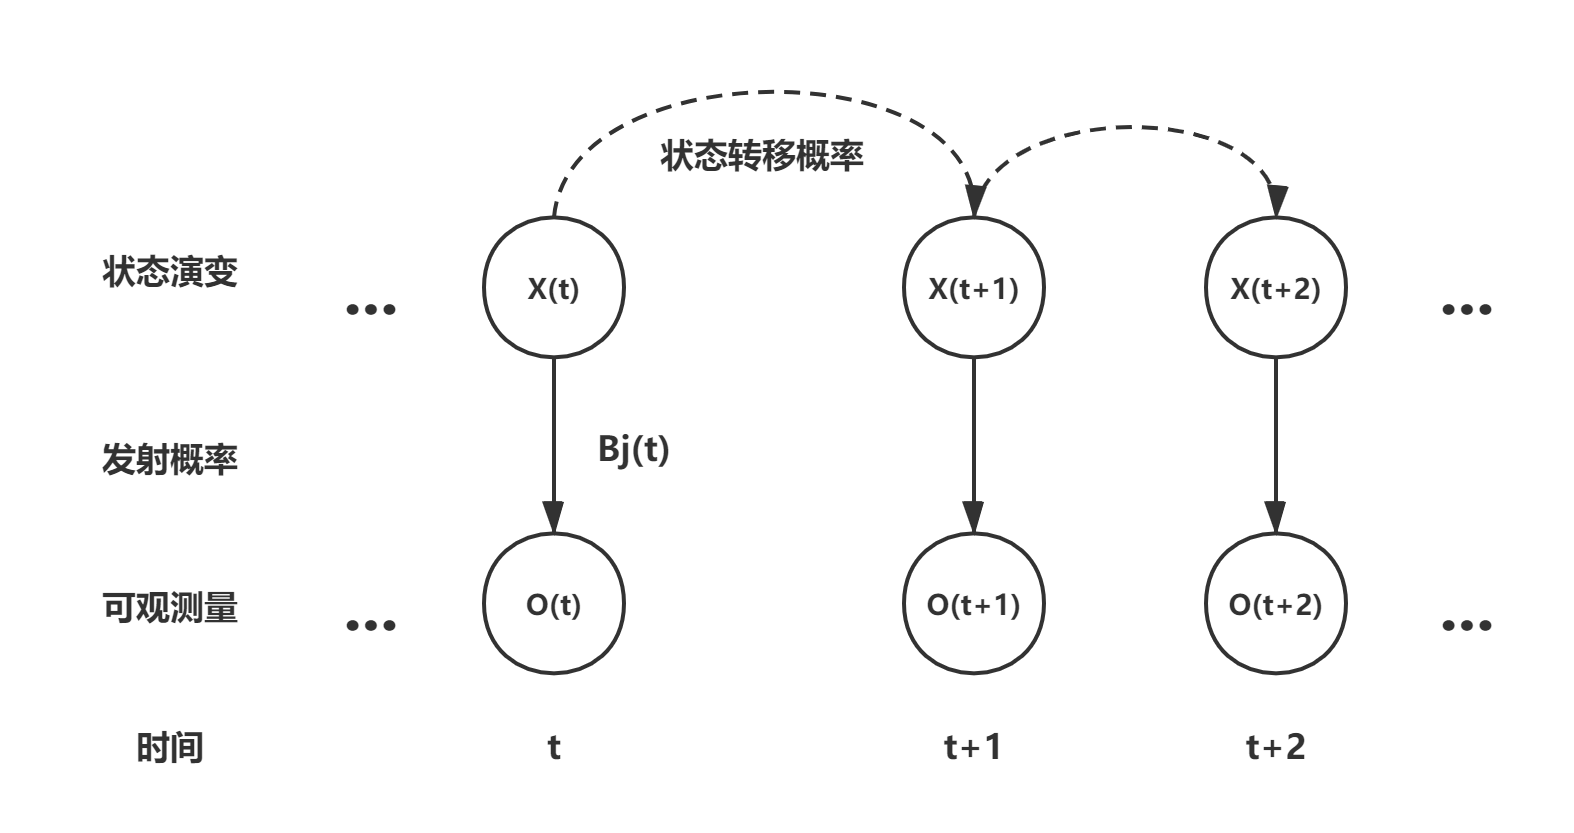
\includegraphics[width=0.8\columnwidth]{HMM.png}
	\caption{HMM 底层架构}
	\label{fig:HMM}
\end{figure}

HMM是一种双随机的有限模型,它可以计算无限数量的可能序列的概率分布。
它用于研究离散时间序列中的观测项。
状态有分配的过渡概率,每个状态根据状态的发射概率输出符号。
图~\ref{fig:HMM}展示了HMM的底层架构。
首先,HMM定义为五元组 $(S, O, A, B, \pi)$:
\begin{itemize}
	\item $S = S_1, S_2, \cdots, S_n$ 表示一组隐状态。
	\item $O(t) = o_1, o_2, \cdots, o_m$ 是一组在每个时间段的 m-可观测符号。
	\item $A$ 表示状态转移概率,并且$A_{ij} = P(X_{t+1} = S_j | X_t = S_i)$。
	\item $B$ 表示符号发射概率,$B_j = b_j(t) = P(O(t)|X(t) = S_j)$,表示从状态 $j$ 发射符号 $O(t)$ 的概率。
	\item $\pi = \{\pi_i = P(X_1 = S_i)| 1 \le i \le n\}$ 表示初始状态概率。
\end{itemize}

隐马尔科夫模型由两个随机过程组成。
第一个随机过程是一个马尔科夫链,它的特征是状态和转换概率。
链的状态在外部是不可见的,因此是 “隐藏的”。
第二个随机过程产生的排放量在每个时刻都是可以观察到的,这取决于一个依赖于状态的概率分布。
需要注意的是,在定义隐藏马尔科夫模型时,“隐藏”这个词指的是马尔科夫链的状态,
而不是模型的参数。HMM的历史由两部分组成。
一方面是马尔科夫过程和马尔科夫链的历史,另一方面是开发隐藏马尔科夫模型所需的算法的历史,以便通过使用计算机或类似的电子设备来解决现代应用科学中的问题。

\section{马尔科夫过程和马尔科夫链的简史}

安德烈-安德烈耶维奇-马尔科夫(1856年6月14日-1922年7月20日)是俄罗斯数学家。他最著名的是他在随机马尔科夫过程理论方面的工作。他的研究领域后来被称为马尔科夫过程和马尔科夫链。安德烈-安德烈耶维奇-马尔科夫在1906年提出了马尔科夫链,他首次使用 "链 "这个术语,得出了随机过程的第一个理论结果。1913年,他计算出俄语的字母序列。Kolmogorov(1931)给出了对可数无限状态空间的泛化。马尔科夫链与布朗运动和厄尔古德假说有关,这两个物理学中的课题在20世纪初很重要。但马尔科夫似乎是出于一种数学动机,即把大数定律扩展到依赖性事件中去追求的。从这种方法中生长出一种一般的统计工具,即所谓随机马尔科夫过程。在一般的数学中,特别是概率论和统计学中,马尔科夫过程可以被认为是一种时变的随机现象,在这种现象中,马尔科夫的特性被满足。

在通常的描述中,一个具有马尔科夫性质或无记忆性的随机过程是指系统的当前状态、未来和过去的条件是独立的 。
马尔科夫过程在概率和统计中以两种方式之一出现。一个随机过程,通过单独的论证定义,可以被证明(数学上)具有马尔科夫属性,并因此具有所有马尔科夫过程的属性,可以由此推导出所有马尔科夫过程。更为重要的实际意义在于,使用马尔科夫性质对某一随机过程成立的假设,来构建该过程的随机模型。在建模方面,假设马尔科夫属性成立是将统计依赖性引入随机过程模型的有限简单方法之一,这种方法允许不同滞后的依赖性强度随着滞后的增加而下降。通常,马尔科夫链这个术语是指具有离散(有限或可计数)状态空间的马尔科夫过程。通常,马尔科夫链的定义是一组离散的时间(即离散时间马尔科夫链),尽管有些学者使用同样的术语,“时间”可以取连续值。

\section{开发隐藏马尔科夫模型需要的算法简史}

随着20世纪40年代计算机科学的大力发展,在约翰-冯-纽曼、图灵、康拉德-祖斯等科学家取得研究成果后,全世界的科学家都在试图寻找算法解决方案,以利用确定性自动和随机性自动来解决现实生活中的许多问题。在经典滤波理论以线性滤波理论为主的基础上,非线性和随机滤波理论变得越来越重要。在20世纪50年代末和60年代,我们可以注意到 "Luenberger-Observer"、"Wiener-Filter"、"Kalman-Filter "或 "Extended Kalman-Filter "以及它的派生品在这一类别中的主导地位。在20世纪中期的同一时期,美国数学家和电子工程师Claude Shannon(1916-2001)在他的论文 《A mathematical theory of communication》中提出了一个非常重要的历史性步骤,他在1948年7月和10月的《贝尔系统技术杂志》上首次发表了两篇论文,这促进了计算机和电气设备对确定性和随机性自动化的实现和集成的需求。为了创建、应用或理解隐藏马尔可夫模型,还需要进一步的算法发展史上的重要内容:

\begin{enumerate}
	\item \textbf{期望最大化(EM)算法}:期望最大化算法的近代史与20世纪初的最大似然的历史有关。R.A.Fisher使最大似然在1912年和1922年之间流行,虽然它已被使用早期的高斯,拉普拉斯,蒂勒,和F.Y.Edgeworth。几年后,1977年Arthur Dempster、Nan Laird和Donald Rubin在《英国皇家统计学会杂志》上的一篇论文中对EM算法进行了解释并命名。他们指出,该方法已经被其他作者 "在特殊情况下多次提出",但1977年的论文概括了该方法并发展了其背后的理论。在统计学中,期望最大化(EM)算法用于寻找概率模型中参数的最大似然估计,其中模型依赖于未观测的潜变量。EM交替执行期望(E)步骤和最大化(M)步骤,前者通过将潜变量当作被观察到的变量来计算似然的期望值,后者通过最大化E步骤上发现的期望似然来计算参数的最大似然估计。然后用M步骤上找到的参数开始另一个E步骤,重复这个过程。在机器学习和计算机视觉中,EM经常被用于数据聚类。在自然语言处理中,该算法的两个突出实例是Baum-Welch算法(又称 "前向-后向")和无监督归纳概率无上下文语法的inside-outside算法。本章以下部分将介绍期望值最大化算法的数学和算法基础,特别是针对HMM应用的算法。
	\item \textbf{鲍姆-韦尔奇算法}:Baum-Welch算法是广义期望最大化(GEM)算法的一种特殊情况(Kouemou 2010,维基百科)。Baum-Welch算法用于寻找隐藏马尔科夫模型(HMM)的未知参数。它利用了前向-后向算法,并以Leonard E. Baum和Lloyd R. Welch命名。Baum-Welch算法的介绍论文之一是1970年提出的 《马尔科夫链的概率函数统计分析中发生的最大化技术》~\cite{GEM}。
	\item \textbf{维特比算法}:Viterbi算法是由Andrew Viterbi在1967年提出的~\cite{Viterbi}。作为一种在嘈杂的数字通信链路上卷积码的解码算法,它是一种动态编程算法。用于寻找最可能的隐藏状态序列,称为Viterbi路径,导致观察到的事件序列。在过去的几年里,这种算法在卷积码解码中得到了普遍的应用,例如用于CDMA和GSM数字蜂窝、拨号调制解调器、卫星、深空通信和802.11无线局域网。现在,它还普遍应用于语音识别应用、关键词定位、计算语言学和生物信息学中。例如,在某些语音转文本识别设备中,声信号被视为观察到的事件序列,而一串文本被认为是声信号的 "隐藏原因"。Viterbi算法可以找到给定声学信号的最可能的文本串。
\end{enumerate}

\section{马尔可夫模型的应用}

隐马尔科夫模型还被用于现代科学或工程应用的许多其他领域,如语音、笔迹、手势识别、语音部分标记、乐谱跟踪、部分放电等时间模式识别。
一些作者甚至使用HMM来解释或预测社会科学或政治领域的个人或群体的行为~\cite{Schrodt2006}。
HMM仍占主导地位的主要应用领域之一是 "语音识别 "领域。
"混淆矩阵 "被广泛使用,以评估基于HMM系统的性能。
矩阵的每一行代表预测类的实例,而每一列代表实际类的实例。混淆矩阵的一个好处是,很容易看出系统是否混淆了两个类(即通常将一个类误标为另一个类)。
当一个数据集是不平衡的,这通常发生在不同类的样本数量差异很大的时候,分类器的错误率不能代表分类器的真实性能。通过一个例子可以很容易理解这一点。如果类1有980个样本,而类2只有20个样本,那么分类器很容易偏向类1。如果分类器将所有的样本都归为1类,那么准确率将达到98\%。这并不能很好地说明分类器的真实性能。分类器对类1的识别率为100\%,但对类2的识别率为0\%。

\chapter{结论}
\label{chap:conclusion}

本文从高斯过程和隐马尔可夫模型两个方向展开,介绍了随机过程在机器学习领域的应用。

\backmatter

% 参考文献
\bibliography{ref/refs}

% 附录
\appendix

\end{document}